\documentclass{scrartcl}

\usepackage[utf8]{inputenc}
\usepackage{color}
\usepackage{xcolor}

\usepackage{graphics}           % Add pictures to the document
\usepackage{graphicx}           % Add pictures to the document
\usepackage{subfigure}          % 2 pictures side by side

\title{Dokumentation ProductAR}
\author{Maximilian Rehberger}
\date{\today}

\setcounter{secnumdepth}{4}
\setcounter{tocdepth}{4}

\definecolor{darkcerulean}{rgb}{0.03, 0.27, 0.49}
\definecolor{frenchblue}{rgb}{0.0, 0.45, 0.73}
\definecolor{babyblueeyes}{rgb}{0.63, 0.79, 0.95}

\addtokomafont{section}{\color{darkcerulean}}
\addtokomafont{subsection}{\color{frenchblue}}
\addtokomafont{subsubsection}{\color{babyblueeyes}}

\graphicspath{ {./img/} }                % Path to images

\begin{document}


\maketitle

\newpage


\renewcommand*\contentsname{}
\section{Inhaltsverzeichnis}
\tableofcontents{}


\newpage

\section{Einleitung}

\subsection{Zweck}

Produkte können zum Beispiel beim Einkaufen mit dem Smartphone gescannt werden und erkannt werden. Informationen werden angezeigt wie zum Beispiel Bilder oder ein Preisvergleich. Mithilfe der App soll man einen Barcode einscannen können und Informationen zu den Produkten erhalten. Weiterhin kann der Nutzer ein Produkt in Augmented Reality (AR) testen und sieht somit wie es in Wirklichkeit aussehen wird, wenn er es kaufen würden.

\newpage

\section{Allgemeine Übersicht}

\subsection{Beschreibung Ausgangssituation}

Es gibt bereits viele Shopping-Apps wie zum Beispiel Ikea, H\&M oder S'Oliver. Das Problem ist, dass jeder am Ende für jedes Geschäft eine eigene App auf dem Smartphone hat. Diese App soll die Möglichkeiten geben mehrere unterschiedliche Produkte in einer App zu speichern und zu verwalten. Also eine App für alle Produkte.

\subsection{Produkteinsatz}

 Die App kann zum Beispiel als Einkaufsliste oder Wunschliste für Produkte eingesetzt werden.
 Darüber hinaus bieten sich noch viele weitere Möglichkeiten.

\subsection{Produktumfeld}

Die App wird hauptsächlich im privaten Umfeld umgesetzt, beim Einkaufen in Geschäften oder Online-Einkauf.

\subsection{Produktfunktionalität}

Scannen von Produkten, Informationen zu Produkten, Preisvergleich, Bilder hochladen für Produkte, Produkte in AR testen.

\subsection{Personas}

\subsubsection{Nutzer}

\subsubsection{Verkäufer}

\subsubsection{Admin}


\newpage

\section{Architekturkonzept und Entwurf}

\subsection{Ursprüngliches Architekturkonzept}

\begin{figure}[h]
\centering
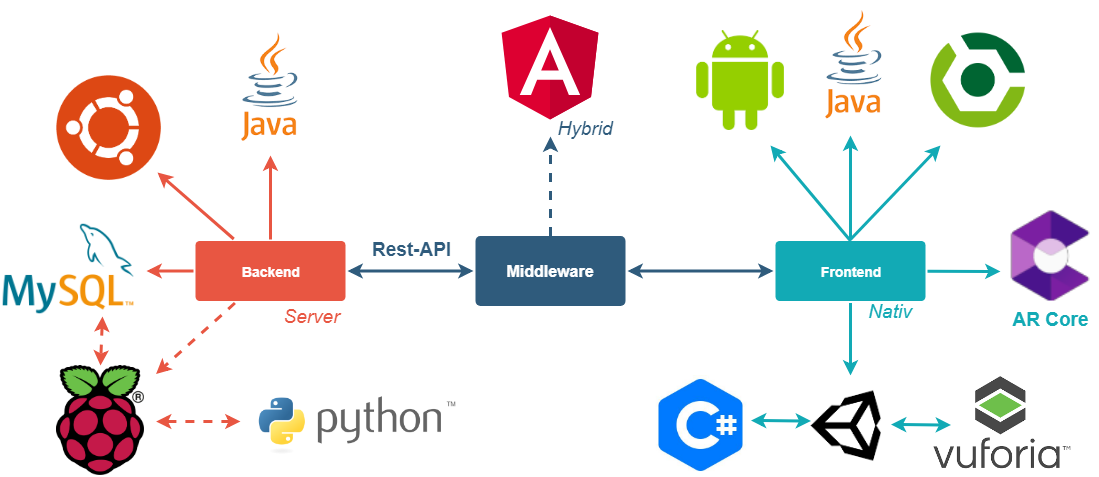
\includegraphics[width=380px]{img/Architekturkonzept.png}
\caption{Ursprüngliches Architekturkonzept}
\end{figure}

\subsection{Aktualisiertes Architekturkonzept}

\begin{figure}[h]
\centering
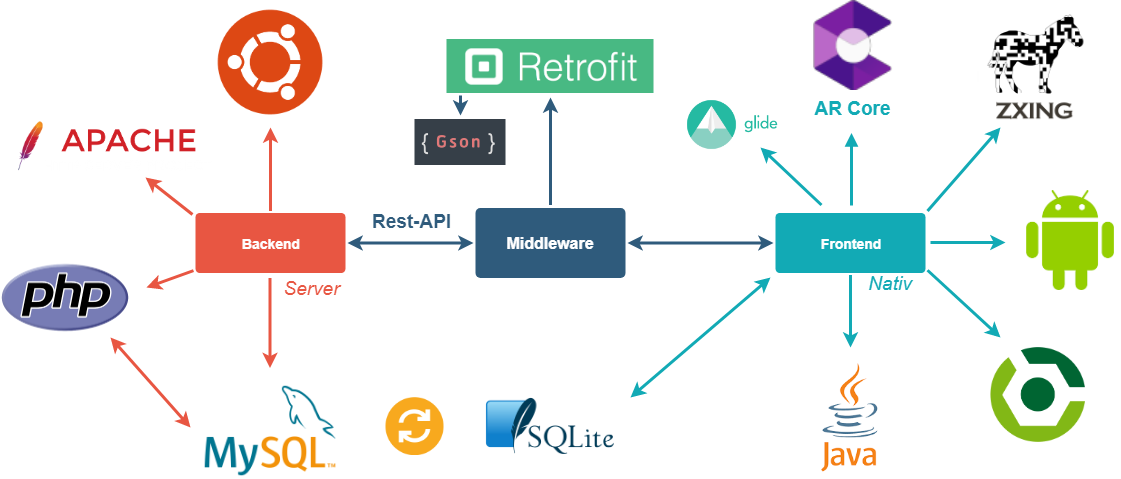
\includegraphics[width=380px]{img/ArchitekturkonzeptNew.png}
\caption{Aktualisiertes Architekturkonzept}
\end{figure}

\newpage

\subsection{Anfängliche Skizze Datenbankentwurf}

\subsubsection{MySQL Datenkbank (Remote)}

Ursprünglich war geplant, dass die Daten ausschließlich auf dem Server in einer MySQL Datenbank gespeichert werden.

\begin{figure}[h]
\centering
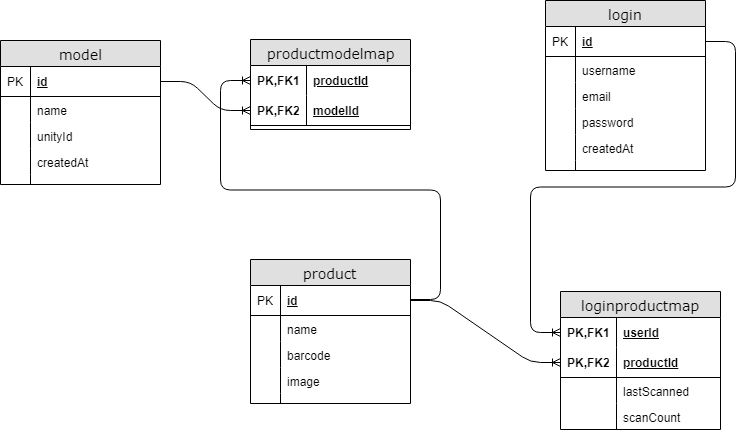
\includegraphics[width=380px]{img/Skizze_Datenbank_1.png}
\caption{Anfängliche Skizze Datenbankentwurf}
\end{figure}

\newpage

\subsection{Anfängliche Skizze Java Klassen}

\begin{figure}[h]
\centering
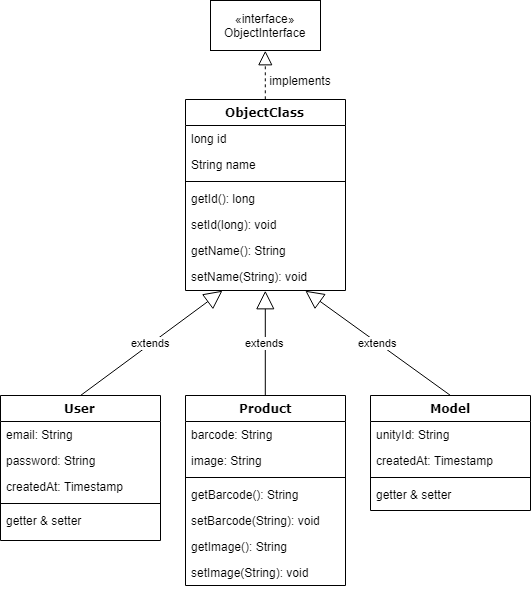
\includegraphics[width=320px]{img/Skizze_Java_1.png}
\caption{Anfängliche Skizze Datenbankentwurf}
\end{figure}

\newpage

\subsection{Endgültige Skizze Datenbankentwurf}

\subsubsection{SQLite Datenbank (Lokal)}

\begin{figure}[h]
\centering
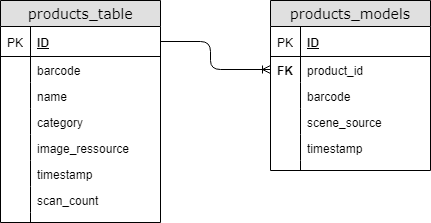
\includegraphics[width=180px]{img/Skizze_Datenbank_SQLite.png}
\caption{Skizze Datenbankentwurf: SQLite}
\end{figure}

\subsubsection{MySQL Datenbank (Remote)}

\begin{figure}[h]
\centering
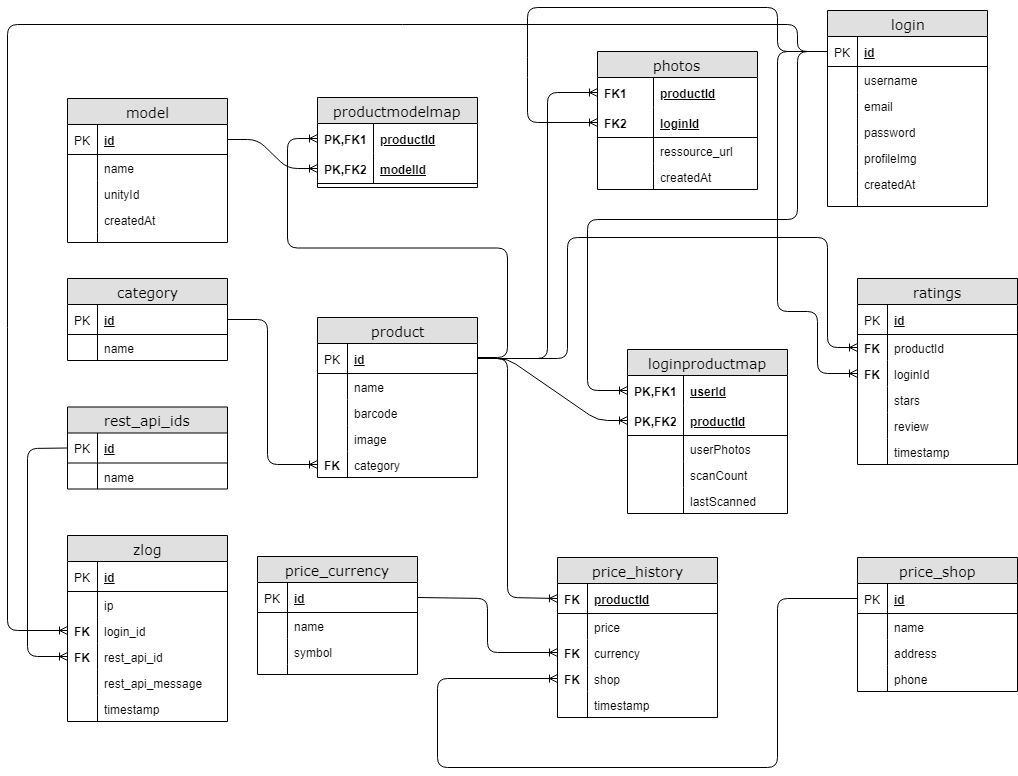
\includegraphics[width=380px]{img/Skizze_Datenbank_2.png}
\caption{Aktualisierte Skizze Datenbankentwurf: MySQL}
\end{figure}

\newpage

\subsection{Endgültige Skizze Java Klassen}

\begin{figure}[h]
\centering
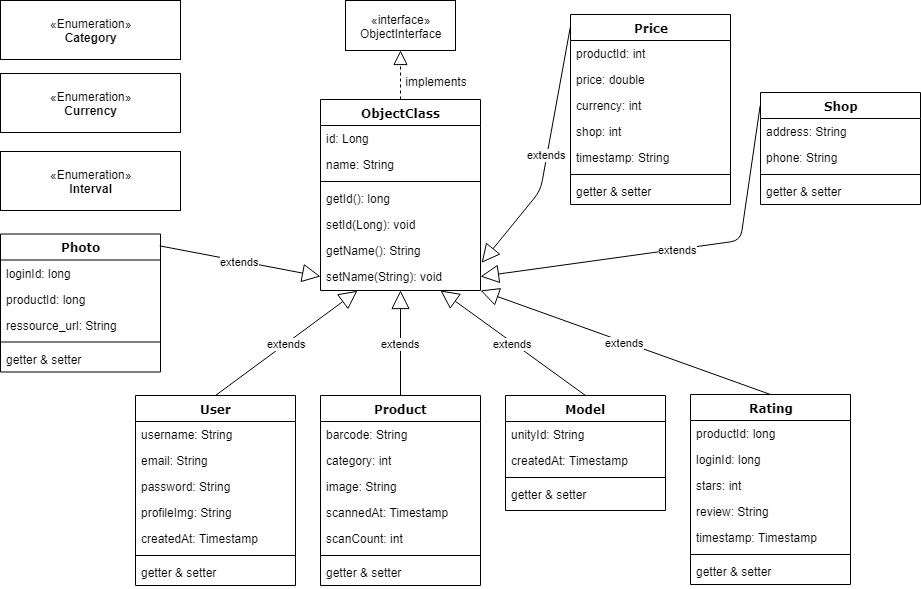
\includegraphics[width=380px]{img/Skizze_Java_New.png}
\caption{Aktualisierte Skizze: Java Klassen}
\end{figure}

\subsection{Übersicht Backend Server}

Der Backend Server ist ein gemieteter Server von Hosteurope. \newline
Produktbezeichnung: "Virtual Server Linux Advanced 8.2". \newline
Dieser hat folgende Linux Version installiert: Ubuntu 16.04.6 LTS. \newline \newline

\noindent Die Technischen Spezifikationen lauten wie folgt: \newline 

\noindent 4 virtuelle Kerne \newline
\noindent 6 GB RAM \newline 
\noindent 200GB SSD \newline 

\noindent Es handelt sich hierbei um einen virtuellen Server, das bedeutet, dass sich der Server mit anderen "Containern" die Hardware eines Servers teilen. % Die Hardware eines großen Server wird auf die Container entsprechend aufgeteilt. % 
\newline

\noindent Der Server hat eine eigene Domain: www.nimoo.de. 

\newpage

\subsection{Übersicht REST API}

Die Rest Schnittstelle wurde mit PHP auf dem Webserver umgesetzt welcher vom Backend Server bereits zur Verfügung gestellt wurde. 
Für jede Ressource existiert ein Pfad, mit entsprechender PHP Datei. \newline 

\noindent Der Hauptpfad für die App auf dem Webserver: "https://www.nimoo.de/apps/productar" \newline

\noindent Folgende Pfade existieren auf dem Webserver: \newline

\noindent ../products/ \newline
\noindent ../products/images/ \newline
\noindent ../products/photos/ \newline
\noindent ../products/prices/ \newline
\noindent ../products/ratings/ \newline
\noindent ../users/ \newline
\noindent ../users/images \newline
\noindent ../models/ \newline

\subsection{Technische Entscheidungen}

\subsubsection{Warum Android?}

Die Entscheidung, die App für Android zu entwickeln wurde getroffen, da Android zumindest in Deutschland einen höheren Marktanteil besitzt als iOS. Vor allem die Studenten der Fakultät Informatik und Wirtschaftsinformatik (FIW) und in der Vertiefung Mobile Solutions benutzen mehrheitlich Android Smartphones. Ein weiterer Grund ist, dass Android Java basiert ist und dafür sehr gut geeignet ist, wenn bereits fortgeschrittene Erfahrungen mit der Programmiersprache Java gegeben sind. Weiterhin gibt es beim Entwickeln keine Mehrkosten, da es bereits viele Open-Source Erweiterungen (Bibliotheken) gibt und Anleitungen, die das Entwickeln weiter vereinfachen.

\subsubsection{Welche Androidversion?}

Als minimal unterstützte Android Version (minSdkVersion) für die App musste die Api 24 (Android 7) verwendet werden. Dies liegt daran, dass die AR Funktionialität mit der Google AR Core Erweiterung erst ab Android Version 7 (Api 24) unterstützt wurde und alle vorherigen Versionen keine Unterstützung haben. Dies hat den Nachteil, dass nur ca. 37,1 \% aller Android Geräte unterstützt werden im Vergleich zu den 95,3 \% die mit Android 4.4 (Api 19) unterstützt würden. 

\subsubsection{Welche Entwicklungsumgebung?}

Zum Entwickeln der App wurde hauptsächlich die Entwicklungsumgebung von Android Studio und IntelliJ genutzt.

\subsubsection{Wieso Google AR Core?}

Googles neuestes Framework für Augmented Reality Anwendungen heist "AR Core". Im Vergleich zu einer AR Anwendung mit Unity lässt es es sich sehr einfach in die App integrieren (Als Fragment oder View in der Aktivity). Weiterhin lassen sich Modelle (.OBJ) sehr einfach mit dem Sceneform Plugin einbinden und bearbeiten. 

\subsubsection{Wieso eine MySQL Datenbank?}

Zum einen war die MySQL Datenbank ebenfalls schon auf dem Backend Server aufgesetzt, somit war keine weitere Konfiguration notwendig. Weiterhin ist es sehr einfach eine Datenbank mit SQL zu erstellen und Abfragen durchzuführen.

\subsubsection{Wieso eine REST API?}

Die Rest API ist die Schnittstelle zwischen der App und der Datenbank auf dem Server. Diese wird benötigt, da man aus Sicherheitsgründen keine direkte Verbindung zwischen App und Datenbank zulassen darf.

\subsubsection{Vergleich mit Alternativlösungen}

\paragraph{Firebase von Google}.\newline

\noindent Die Backendlösung von Google ist "FireBase" und wäre erheblich einfacher umzusetzten und hätte ebenfalls den Vorteil, dass kein externer Server benötigt wird. Warum wurde diese Lösung in diesem Projekt jedoch nicht verwendet? Die Datenbank enthält sensible Daten, wie zum Beispiel Nutzerdaten. Diese sollen nicht an Google gesendet werden.

\paragraph{Alternative Datenbankmodelle}.\newline

\noindent PostgreSQL und MongoDB.

\newpage

\section{Technische Dokumentation}

Die Dokumentation der einzelnen Java Klassen befindet sich im generierten JavaDoc Verzeichnis. Die nachfolgende Dokumentation wurde aus den JavaDoc Kommentaren übernommen.

\subsection{Android Manifest}

\subsection{Java Interfaces}

\subsubsection{ObjectInterface}

Das Interface "ObjectInterface" definiert die Vorgaben, welches ein Objekt erfüllen muss. Ein Objekt benötigt eine id als eindeutigen Identifizierer und einen Namen. Entsprechende Getter und Setter sind hier definiert.

\subsubsection{ScanResultReceiver}

Das Interface "ScanResultReceiver" definiert die Methoden, welche nach dem Scannen eines Barcodes ausgeführt werden. \newline

\noindent\textbf{Methode scanResultData(NoScanResultException noScanData)}\newline Die Methode "scanResultData" wird aufgerufen, wenn das Scannen des Barcodes fehlgeschlagen ist.\newline

\noindent\textbf{Methode scanResultData(java.lang.String codeFormat, java.lang.String codeContent)}\newline Die Methode "scanResultData" wird nach dem erfolgreichen Scannen des Barcodes aufgerufen.

\subsubsection{IRetrofitCRUD}

Das Interface "IRetrofitCRUD" definiert die Methoden, welche aufgerufen werden um über Retrofit Anfragen an den Server zu stellen.

\subsubsection{JsonPlaceHolderApi}

Das Interface "JsonPlaceHolderApi" ist die direkte Schnittstelle zwischen Retrofit und dem Zielserver. Verwendete HTTP Verbs: GET und POST.

\subsection{Java Klassen}

\subsubsection{Objekt Klassen}

\paragraph{Object Class (Abstract)}

Die Klasse "ObjectClass" ist eine abstrakte Klasse, welche die benötigten Methoden für ein Objekt implementiert.

\paragraph{Product}

Die Klasse "Product" stellt die Objektklasse für ein Produkt dar. Ein Produkt ist gleichzeitig ein Objekt. Hier werden wichtige Methoden und Konstruktoren implementiert. Die Werte können über Getter und Setter Methoden abgefragt werden.

\paragraph{User}

Die Klasse "User" stellt die Objektklasse für einen Benutzer dar. Ein Benutzer ist gleichzeitig ein Objekt. Hier werden wichtige Methoden und Konstruktoren implementiert. Die Werte können über Getter und Setter Methoden abgefragt werden.

\paragraph{Model}

Die Klasse "Model" stellt die Objektklasse für ein (AR) Model dar. Ein Model ist gleichzeitig ein Objekt. Hier werden wichtige Methoden und Konstruktoren implementiert. Die Werte können über Getter und Setter Methoden abgefragt werden.

\paragraph{Photo}

Die Klasse "Photo" stellt die Objektklasse für ein Foto dar. Ein Foto ist gleichzeitig ein Objekt. Hier werden wichtige Methoden und Konstruktoren implementiert. Die Werte können über Getter und Setter Methoden abgefragt werden.

\paragraph{Price}

Die Klasse "Price" stellt die Objektklasse für einen Preis dar. Ein Preis ist gleichzeitig ein Objekt. Hier werden wichtige Methoden und Konstruktoren implementiert. Die Werte können über Getter und Setter Methoden abgefragt werden.

\paragraph{Shop}

Die Klasse "Shop" stellt die Objektklasse für einen Shop dar. Ein Shop ist gleichzeitig ein Objekt. Hier werden wichtige Methoden und Konstruktoren implementiert. Die Werte können über Getter und Setter Methoden abgefragt werden.

\paragraph{Category (Enum)}

Die Enumklasse "Category" beinhaltet die Produktkategorien. Es gibt folgende Kategorien: Accessoires, Auto, Baumarkt, Beauty, Bücher, Computer, Drogerie, Elektronik, Filme, Garten, Haushalt, Kleidung, Lebensmittel, Möbel, Musik, Schuhe, Serien, Spiele, Spielzeug, Sport.

\paragraph{Currency (Enum)}

Die Enumklasse "Currency" beinhaltet die aktuell unterstützten Währungen. In diesem Fall: Dollar und Euro.

\paragraph{Interval (Enum)}

Die Enumklasse "Interval" beinhaltet die Möglichkeiten für ein Updateinterval der Benachrichtigungen. Folgende Intervalle sind für Benachrichtigungen möglich: Täglich, Wöchentlich, Monatlich.

\newpage

\subsubsection{Aktivity Klassen}

\paragraph{MainActivity}

\noindent Die Klasse "MainActivity" wird beim Starten der App ausgeführt, direkt nach dem "SplashScreen". Es können Barcodes gescannt und danach das Ergebnis angezeigt werden.\newline

\noindent\textbf{Methode onCreate(android.os.Bundle savedInstanceState)}

\noindent Die Methode "onCreate" wird beim Start der Activity ausgeführt. Hier werden Werte initialisiert, zum Beispiel TextViews oder Buttons. Es wird eine Datenbankverbindung zur lokalen SQLite Datenbank initialisiert. Ein OnClickListener wird für den Button "btn\_scan\_now" initialisiert. Für Android Versionen größer 23 (ab 24) wird ein NetworkMonitor Receiver erzeugt.\newline

\noindent\textbf{Methode onCreateOptionsMenu(android.view.Menu menu)}

\noindent Die Methode "onCreateOptionsMenu" erzeugt das Menü für die AktionsLeiste Es wird zuerst überprüft ob der Nutzer eingeloggt ist. Nutzername und Password werden in einem User Objekt gespeichert. Das Menü "menu\_loggedin" wird hier verwendet. Der Nutzername wird in das Feld "action\_username" eingetragen und ein OnClickListener erstellt mit der Methode "goToProfile". Für den Logout Button wird ebenfalls ein OnClickListener erstellt, welcher den Nutzer ausloggt. Ist der Nutzer allgemein nicht eingloggt, so wird stattdessen das Standardmenü geladen. \newline

\noindent\textbf{Methode onDestroy()}

\noindent Die Methode "onDestroy" wird beim verlassen der Activity ausgeführt. \newline

\noindent\textbf{Methode onOptionsItemSelected(android.view.MenuItem item)}

\noindent Die Methode "onOptionsItemsSelected" wird ausgeführt, wenn ein Menüelement ausgewählt wurde. Je nachdem um welches Element es sich handelt werden unterschiedliche Aktionen ausgeführt. Bei "action\_login": Wenn eingeloggt, dann wird mann zum Profil weitergeleitet. Wenn nicht eingeloggt, dann wird man zum Login weitergeleitet. Bei "action\_settings": Man wird zu den Einstellungen weitergeleitet. Bei "action\_info": Man wird zu den Informationen über die App weitergeleitet. Bei "action\_close": Die App wird beendet. \newline

\noindent\textbf{Methode scanNow(android.view.View view)}

\noindent Die Methode "scanNow" wird ausgeführt, wenn der Button "btn\_scan\_now" geklickt wurde. Es wird ein ScanFragment erzeugt, welches als nächstes geöffnet wird. Die Kamera wird aktiviert und der Barcode Scanner wird initialisiert. \newline

\noindent\textbf{Methode scanResultData(java.lang.String codeFormat, java.lang.String codeResult)}

\noindent Die Methode "scanResultData" wird ausgeführt, wenn der Barcode Scanner einen Code erfolgreich gescannt hat. Zuerst wird geprüft ob der barcode existiert (!nullCheck) Als nächstes beginnt die Ladeanimation (loadingStart()) Es wird versucht den Barcode in eine Long Variable umzuwandeln um zu prüfen ob der Barcode numerisch ist. Wenn keine NumberFormatException abgefangen worden ist wird in der lokalen SQLite Datenbank nach einem Barcode gesucht, welcher schon existiert. Von diesem wird der Name und das Bild benötigt. Wenn kein Barcode lokal existiert, dann wird eine Abfrage mit Retrofit ausgeführt, welche prüft ob ein Produkt mit dem Barcode in der MySQL Datenbank auf dem Server vorhanden ist. Sollte ein Produkt auf dem Server existieren, dann wird es in die Lokale Datenbank übertragen Es wird zusätzlich überprüft ob ein Model zu dem Produkt in der lokalen Datenbank existiert, wenn nicht, dann wird eins vom Server angefragt und in die Datenbank übertragen. Wenn kein Produkt auf dem Server existiert, dann wird die Methode "createNewBarcode" aufgerufen um einen neues Produkt auf dem lokalen Gerät zu erstellen. Wenn der Barcode bereits lokal existiert, wird der Zeitstempel für das Produkt aktualisiert und die Anzahl der Scans um 1 inkrementiert. Außerdem wird das Produkt als "bereit zum Synchronisieren" gekennzeichnet Das Ergebnis für das Bild und den Namen aus der lokalen Datenbank wird nun angezeigt und in die davor vorgesehenen Views geladen. Abschließend wird die Ladeanimation wieder beendet (loadingEnd()) \newline

\noindent\textbf{Methode scanResultData(NoScanResultException noScanData)}

\noindent Für den Fall das der Scan fehlgeschlagen ist. \newline

\noindent\textbf{Methode createNewBarcode(java.lang.String newBarcode)}

\noindent Die Methode "createNewBarcode" leitet auf die "CreateProductActivity" weiter und übergibt dieser den gescannten Barcode. \newline

\noindent\textbf{Methode goToProfile()}

\noindent Die Methode "goToProfile" leitet einen zum Nutzerprofil weiter. \newline

\noindent\textbf{Methode loadingStart()}

\noindent Die Methode "loadingStart" startet die Ladeanimation. \newline

\noindent\textbf{Methode loadingEnd()}

\noindent Die Methode "loadingEnd" beendet die Ladeanimation. \newline

\newpage

\paragraph{SplashScreen}

Die "SplashScreen" Activity wird ganz am Anfang gestartet. Es wird ein Drawable angezeigt. Anschließend wird auf die "MainActivity" weitergeleitet. \newline

\noindent\textbf{Methode onCreate(android.os.Bundle savedInstanceState)}

\noindent Die Methode "onCreate" initialisiert Variablen und ruft die Methode "scheduleJob" auf. Weiterhin wird ein CountdownTimer eingestellt, welcher beim Ablauf auf die "MainActivity" weiterleitet. \newline

\noindent\textbf{Methode scheduleJob()}

\noindent Die Methode "scheduleJob" plant einen Job, welcher im Hintergrund ausgeführt werden soll. Dieser ist notwendig um den Nutzer in einem bestimmten Zeitinterval über Neuigkeiten oder Aktualisierungen informieren zu können. In diesem Fall wird der Nutzer über neue Angebote zu seinen Produkten informiert. \newline

\noindent\textbf{Methode cancelJob()}

\noindent Die Methode "cancelJob" entfernt den geplanten Job wieder. \newline

\newpage

\paragraph{ProductArActivity} Die Klasse "ProductArActivity" wird ausgeführt, wenn der Nutzer ein Produkt in AR testen möchte. Das Produkt kann auf eine beliebige gefundene Fläche in AR platziert werden. Wenn kein Produkt zum Testen ausgewählt wurde, dann erscheint ein leerer Einkaufswagen als Model zum Testen. \newline

\noindent\textbf{Methode onCreate(android.os.Bundle savedInstanceState)} 

\noindent Die Methode "onCreate" wird beim Start der Activity ausgeführt. Wenn ein Barcode von einem Produkt an die Activity übergeben wurde, dann wird das Model aus der lokalen SQLite Datenbank abgefragt, ansonsten wird ein Standardmodel verwendet. Wenn die Einstellung "AR Marker" nicht aktiv ist, dann geht es weiter. Das ArFragment wird initialisiert und es wird ein OnTapArPlaneListener erstellt, welcher ausgeführt wird, wenn man auf eine gefundene AR Fläche tippt. An dieser Stelle wird dann ein Ankerpunkt erzeugt, auf welchen das Model platziert wird.\newline

\noindent\textbf{Methode addModelToScene(com.google.ar.core.Anchor anchor, \newline com.google.ar.sceneform.rendering.ModelRenderable modelRenderable)} 

\noindent Die Methode "addModelToScene" fügt der Scene das Model hinzu. \newline 



\paragraph{ProductScanActivity} Die Klasse "ProductScanActivity" wird ausgeführt, wenn der Nutzer ein Produkt in AR testen möchte. Anders als bei der "ProductArActivity" wird das Produkt nur auf einen vorher generierten QR Code platziert, welcher dem Namen oder den Barcode des Produkts entspricht. Dies geschieht automatisch. Wenn kein Produkt zum Testen ausgewählt wurde, dann erscheint ein leerer Einkaufswagen als Model zum Testen. \newline

\noindent\textbf{Methode onCreate(android.os.Bundle savedInstanceState)}

\noindent Die Methode "onCreate" wird beim Starten der Activity ausgeführt. Wenn ein Barcode von einem Produkt an die Activity übergeben wurde, dann wird das Model aus der lokalen SQLite Datenbank abgefragt, ansonsten wird ein Standardmodel verwendet. Wenn die Einstellung "AR Marker" aktiv ist, dann geht es weiter. In diesem Fall wird ein CustomArFragment initialisiert und ein OnUpdateListener hinzugefügt. \newline

\noindent\textbf{Methode onUpdate(com.google.ar.sceneform.FrameTime frameTime)}

\noindent Die Methode "onUpdate" wird aufgerufen, wenn eine Aktualisierung in der AR Scene stattgefunden hat. Für jedes Image Target wird überprüft, ob es in der Scene getrackt wird. Wird ein Image Target getrackt, dann wird überprüft ob der key name des getrackten Images mit denen der festgelegten Image Targets übereinstimmt. Wenn es übereinstimmt, dann wird eine Toast Nachricht angezeigt. Anschließend wird ein Ankerpunkt in der Mitte des Image Targets platziert und die Methode "createModel" aufgerufen und dieser den Ankerpunkt übergeben. \newline

\noindent\textbf{Methode setupDatabase(com.google.ar.core.Config config, \newline com.google.ar.core.Session session)}

\noindent Die Methode "setupDatabase" erzeugt die AugmentedImageDatabase, in welcher die Bilder sind, welche in der AR Scene getrackt werden müssen. Es werden 3 Image Targets hinzugefügt. 1. Image Target: QR Code: "fox" 2. Image Target: QR Code: Name vom Produkt 3. Image Target: QR Code: Barcode vom Produkt. \newline

\noindent\textbf{Methode createModel(com.google.ar.core.Anchor anchor)}

\noindent Die Methode "createModel" erzeugt das Model auf den Ankerpunkt. \newline

\noindent\textbf{Methode 	placeModel(com.google.ar.sceneform.rendering.ModelRenderable \newline modelRenderable, com.google.ar.core.Anchor anchor)}

\noindent Die Methode "placeModel" platziert das Model. \newline



\paragraph{CaptureActivityPortrait}

Die Klasse "CaptureActivityPortrait" ist dafür da, dass der Barcode Scanner im Hochkant Format ausgeführt wird und nicht beim Drehen des Devices mitrotiert. \newline 


\paragraph{LastScannedProductsActivity}

Die Klasse "LastScannedProductsActivity" zeigt die zuletzt gescannten Produkte der Reihenfolge absteigend an. Es existiert eine "ListView" in der die Objekte geladen werden. \newline

\noindent\textbf{Methode onCreate(@Nullable android.os.Bundle savedInstanceState)}

\noindent Die Methode "onCreate" wird beim Start der Activity ausgeführt. Hier werden wichtige Werte initialisiert zum Beispiel eine ListView. Es wird eine Datenbankabfrage auf die Lokale SQLite Datenbank erzeugt, welche alle lokal gespeicherten Produkte nach Zeitstempel sortiert (neuesten zuerst) wieder zurück gibt. Wenn es keine Produkte gibt, so wird eine TextView "noContentText" sichtbar gemacht. Ansonsten werden die gefundenen Produkte nach und nach erzeugt und einer Liste hinzugefügt. Es wird ein ProductListAdapter mit dieser Liste erzeugt, welcher für die ListView gesetzt wird. Außerdem wird ein OnItemClickListener für jedes Item der ListView erzeugt, welcher auf die "ProductDetailActivity" für das Produkt weiterleitet und dieser den Barcode des Produkts übergibt. \newline

\noindent\textbf{Methode onCreateOptionsMenu(android.view.Menu menu)}

\noindent Die Methode onCreateOptionsMenu erzeugt das Menü für die AktionsLeiste Es wird zuerst überprüft ob der Nutzer eingeloggt ist. Nutzername und Password werden in einem User Objekt gespeichert. Das Menü "menu\_loggedin" wird hier verwendet. Der Nutzername wird in das Feld "action\_username" eingetragen und ein OnClickListener erstellt mit der Methode "goToProfile". Für den Logout Button wird ebenfalls ein OnClickListener erstellt, welcher den Nutzer ausloggt. Ist der Nutzer allgemein nicht eingloggt, so wird stattdessen das Standardmenü geladen. \newline

\noindent\textbf{Methode onOptionsItemSelected(android.view.MenuItem item)} 

\noindent Die Methode "onOptionsItemsSelected" wird ausgeführt, wenn ein Menüelement ausgewählt wurde. Je nachdem um welches Element es sich handelt werden unterschiedliche Aktionen ausgeführt. Bei "action\_login": Wenn eingeloggt, dann wird mann zum Profil weitergeleitet. Wenn nicht eingeloggt, dann wird man zum Login weitergeleitet. Bei "action\_settings": Man wird zu den Einstellungen weitergeleitet. Bei "action\_info": Man wird zu den Informationen über die App weitergeleitet. Bei "action\_close": Die App wird beendet. \newline

\noindent\textbf{Methode addNewProduct()} 

\noindent Die Methode "addNewProduct" setzt einen OnClickListener auf den ActionButton "addNewProductActionButton" welcher auf die "CreateProductActivity" weiterleitet. \newline

\noindent\textbf{Methode goToProfile()} 

\noindent Die Methode "goToProfile" leitet einen zum Nutzerprofil weiter. \newline

\paragraph{CreateProductActivity}

Die Klasse "CreateProductActivity" ist dazu da um ein neues Produkt zu erstellen, welches in der lokalen SQLite Datenbank abgespeichert wird. \newline

\noindent\textbf{Methode onCreate(android.os.Bundle savedInstanceState)} 

\noindent Die Methode "onCreate" wird beim Starten der Activity ausgeführt. Zunächst wird geprüft ob ein Barcode mit übergeben wurde. Wenn ein Barcode existiert, dann wird dem EditText "editBarcode" dieser als Text gesetzt. Es werden Werte initialisiert, zum Beispiel Buttons, TextViews oder EditText Felder. \newline

\noindent\textbf{Methode onCreateOptionsMenu(android.view.Menu menu)} 

\noindent Die Methode onCreateOptionsMenu erzeugt das Menü für die AktionsLeiste Es wird zuerst überprüft ob der Nutzer eingeloggt ist. Nutzername und Password werden in einem User Objekt gespeichert. Das Menü "menu\_loggedin" wird hier verwendet. Der Nutzername wird in das Feld "action\_username" eingetragen und ein OnClickListener erstellt mit der Methode "goToProfile". Für den Logout Button wird ebenfalls ein OnClickListener erstellt, welcher den Nutzer ausloggt. Ist der Nutzer allgemein nicht eingloggt, so wird stattdessen das Standardmenü geladen. \newline

\noindent\textbf{Methode onOptionsItemSelected(android.view.MenuItem item)} 

\noindent Die Methode "onOptionsItemsSelected" wird ausgeführt, wenn ein Menüelement ausgewählt wurde. Je nachdem um welches Element es sich handelt werden unterschiedliche Aktionen ausgeführt. Bei "action\_login": Wenn eingeloggt, dann wird mann zum Profil weitergeleitet. Wenn nicht eingeloggt, dann wird man zum Login weitergeleitet. Bei "action\_settings": Man wird zu den Einstellungen weitergeleitet. Bei "action\_info": Man wird zu den Informationen über die App weitergeleitet. Bei "action\_close": Die App wird beendet. \newline

\noindent\textbf{Methode AddDataListener()} 

\noindent Die Methode "AddDataListener" erstellt einen OnClickListener für den Button "btnAdd". Es werden die Produktdaten in die lokale SQLite Datenbank übertragen. Zuerst wird überprüft ob das Feld für den Barcode leer ist. Ist dies der Fall wird eine aussagekräftige Fehlermeldung in ein TextView geladen. Ansonsten wird als nächstes versucht den Barcode in eine Long Variable umzuwandeln. Dies dient dazu, herauszufinden ob der Barcode numerisch ist. Ist dies nicht der Fall, wird eine aussagekräftige Fehlermeldung in ein TextView geladen. Als nächstes wird überprüft ob der Barcode bereits in der lokalen SQLite Datenbank oder in der Datenbank auf dem Server schon existiert. Ist dies der Fall, wird eine aussagekräftige Fehlermeldung in ein TextView geladen. Ist der Barcode noch nicht vorhanden so geht es weiter. Als nächstes wird überprüft ob der Name des Produkts leer ist. Ist dies der Fall, wird eine aussagekräftige Fehlermeldung in ein TextView geladen. Weiterhin wird überprüft ob der Bild URL leer ist. Ist dies der Fall, wird eine aussagekräftige Fehlermeldung in ein TextView geladen. Sind alle Produktdaten korrekt, dann werden diese in die lokale SQLite Datenbank übertragen. Wenn diese erfolgreich übertragen wurden, werden die Daten mit dem Server synchronisiert. Außerdem wird eine aussagekräftige Toast Nachricht erzeugt. Zum Schluss wird der Nutzer zurück zur "MainActivity" geleitet, falls er von da gekommen ist.\newline 

\noindent\textbf{Methode imageUploadListener()} 

\noindent Die Methode "imageUploadListener" setzt einen OnClickListener für den Button "btnImgUpload" und fragt die Erlaubnis für den Dateizugriff auf die Fotogalerie an.\newline 

\noindent\textbf{Methode takePhotoListener()} 

\noindent Die Methode "takePhotoListener" setzt einen OnClickListener für den Button "btnTakePhoto" und fragt die Erlaubnis für die Benutzung der Kamera an. \newline

\noindent\textbf{Methode imageUploadListener()} 

\noindent Die Methode "imageUploadListener" setzt einen OnClickListener für den Button "btnImgUpload" und fragt die Erlaubnis für den Dateizugriff auf die Fotogalerie an. \newline

\noindent\textbf{Methode requestCameraPermissions()} 

\noindent Die Methode "requestCameraPermissions" fragt die Erlaubnis für den Zugriff auf die Kamera an. Diese wird benötigt um Fotos vom Produkt zu machen und diese hochzuladen. \newline

\noindent\textbf{Methode deleteBarcodesListener()} 

\noindent Die Methode "deleteBarcodesListener" setzt einen OnClickListener auf den Button "btnDelete". Dieser ist standardgemäß ausgeblendet. Es werden alle Produkte aus der Datenbank gelöscht. \newline 

\noindent\textbf{Methode fillSpinnerWithCategoryData()} 

\noindent Die Methode "fillSpinnerWithCategoryData" füllt das DropDown Menü mit den Produktkategorien. Zuerst werden die Kategorien abgefragt und in ein String-Array gespeichert. Der aktuelle "categoryString" entspricht dem ersten Element des Arrays. Als nächstes wird ein ArrayAdapter erzeugt mit diesem String Array. Der ArrayAdapter wird anschließend für den "categorySpinner" gesetzt. Zum Schluss wird noch ein OnItemSelectedListener definiert, welcher den "categoryString" für jedes ausgewählte Element neu setzt. \newline

\noindent\textbf{Methode requestFilePermission()} 

\noindent Die Methode "requestFilePermissions" fragt die Erlaubnis für den Zugriff auf das Dateisystem an. Diese wird benötigt um die lokale Fotogalerie zu öffnen. \newline

\noindent\textbf{Methode onRequestPermissionsResult(int requestCode, \newline           java.lang.String[] permissions, int[] grantResults)} 

\noindent Die Methode "onRequestPermissionsResult" wird ausgeführt, wenn die Erlaubnis erteilt oder verweigert wurde. Wenn die Erlaubnis für das Dateisystem erteilt wurde, wird die Fotogalerie geöffnet. Wenn die Erlaubnis für die Kamera erteilt wurde, wird die Kamera geöffnet. \newline 

\noindent\textbf{Methode openCamera()} 

\noindent Die Methode "openCamera" erzeugt einen neuen Intent (ACTION\_IMAGE\_CAPTURE). Bevor die Kamera geöffnet wird, wird mithilfe der Methode "createPhotoFile" ein neuer Dateipfad für das Foto ezeugt, welches die Kamera aufnehmen wird, damit es lokal gespeichert werden kann. Anschließend wird der Pfad als URI an den Intent mit übergeben, welcher anschließend gestartet wird. Der Nutzer wird zur Kamera weitergeleitet. \newline

\noindent\textbf{Methode openFilePicker()} 

\noindent Die Methode "openFilePicker" öffnet die lokale Bildergalerie, also die Fotos welche auf dem Gerät gespeichert sind. Dazu wird ein neuer Intent erstellt (ACTION\_PICK) mit dem Type "image/*". Dieser wird anschließend gestartet. \newline

\noindent\textbf{Methode createPhotoFile()} 

\noindent Die Methode "createPhotoFile" erzeugt einen neuen Dateipfad für das Bild, welches von der Kamera aufgenommen wird. Dieser setzt sich aus dem Standardpfad für Bilder und dem Dateinamen zusammen. Der Dateiname wird mit "IMG\_" + "yyyMMdd\_HHmmss" + ".jpg" erzeugt. \newline

\noindent\textbf{Methode onActivityResult(int requestCode, int resultCode, \newline android.content.Intent data)} 

\noindent Die Methode "onActivityResult" wird ausgeführt, wenn der Nutzer wieder von der Kamera oder der Galerie zurück geleitet wurde. Es wird zunächst überprüft ob der Nutzer von der Kamera oder von der Galerie zurück geleitet wurde. Wenn der Nutzer von der Galerie zurück geleitet wurde, dann wird überprüft ob die übermittelten Daten nicht null sind (nullCheck()) und die URI erstellt, welche dem ausgewählten Bild entspricht. Wenn der Nutzer von der Kamera zurück geleitet wurde, dann ist der entsprechende Bildpfad, derjenige, welcher vor dem Aufruf der Kamera mit der Methode "createPhotoFile" erzeugt wurde. In beiden Fällen wird der Bildpfad in der Variable "imgUplPath" gespeichert. \newline

\noindent\textbf{Methode closeKeyboard()} 

\noindent Die Methode "closeKeyboard" schließt die Onscreen Tastatur. \newline 

\noindent\textbf{Methode goToProfile()} 

\noindent Die Methode "goToProfile" leitet einen zum Nutzerprofil weiter. \newline

\noindent\textbf{Methode goToMainActivity()} 

\noindent Die Methode "goToMainActivity" leitet einen zur "MainActivity" weiter. \newline

\newpage

\paragraph{ProductDetailActivity} Die Klasse "ProductDetailActivity" zeigt alle Einzelheiten zu einem Produkt an. \newline

\noindent\textbf{Methode onCreate(android.os.Bundle savedInstanceState)} 

\noindent Die Methode "onCreate" wird beim Start der Activity ausgeführt. Hier werden Werte initialisiert, zum Beispiel TextViews und Buttons. Der Barcode, welcher von der vorherigen Activity übergeben wurde, wird hier wieder von den Intent Extras übergeben. Mithilfe des Barcodes werden aus der lokalen SQLite Datenbank alle wichtigen Informationen zum Produkt abgefragt. Wenn keine Informationen gefunden werden, wird eine aussagekräftige Fehlermeldung angezeigt. Ansonsten werden die zum Produkt gefundenen Informationen in die TextViews geladen. Das Bild wird in die ImageView geladen. Es wird zusätzlich ein zweites Bild erzeugt, welches dem Barcode entspricht. Für die Buttons werden Methoden aufgerufen, welche OnClickListener festlegen. Wenn der Nutzer eingeloggt ist, dann werden die Buttons für das Hochladen von Fotos mithilfe der Kamera oder der lokalen Fotogalerie initialisiert. Am Ende wird der Preis mit der Methode "fetchCurrentPrice" abgefragt. \newline

\noindent\textbf{Methode onCreateOptionsMenu(android.view.Menu menu)} 

\noindent Die Methode onCreateOptionsMenu erzeugt das Menü für die AktionsLeiste Es wird zuerst überprüft ob der Nutzer eingeloggt ist. Nutzername und Password werden in einem User Objekt gespeichert. Das Menü "menu\_loggedin" wird hier verwendet. Der Nutzername wird in das Feld "action\_username" eingetragen und ein OnClickListener erstellt mit der Methode "goToProfile". Für den Logout Button wird ebenfalls ein OnClickListener erstellt, welcher den Nutzer ausloggt. Ist der Nutzer allgemein nicht eingloggt, so wird stattdessen das Standardmenü geladen. \newline

\noindent\textbf{Methode onOptionsItemSelected(android.view.MenuItem item)} 

\noindent Die Methode "onOptionsItemsSelected" wird ausgeführt, wenn ein Menüelement ausgewählt wurde. Je nachdem um welches Element es sich handelt werden unterschiedliche Aktionen ausgeführt. Bei "action\_login": Wenn eingeloggt, dann wird mann zum Profil weitergeleitet. Wenn nicht eingeloggt, dann wird man zum Login weitergeleitet. Bei "action\_settings": Man wird zu den Einstellungen weitergeleitet. Bei "action\_info": Man wird zu den Informationen über die App weitergeleitet. Bei "action\_close": Die App wird beendet. \newline

\noindent\textbf{Methode productPhotosActionListener()} 

\noindent Die Methode "productPhotosActionListener" setzt einen OnClickListener für den Button "buttonProductPhotos", welcher den Nutzer zu den Produktfotos weiterleitet und den Barcode des Produkts mit übergibt. \newline

\noindent\textbf{Methode btnTakePhotoActionListener()} 

\noindent Die Methode "btnTakePhotoActionListener" setzt einen OnClickListener für den Button "btnTakePhoto" und fragt die Erlaubnis für die Benutzung der Kamera an. \newline

\noindent\textbf{Methode btnUploadImageActionListener()} 

\noindent Die Methode "btnUploadImageActionListener" setzt einen OnClickListener für den Button "btnImageUpload" und fragt die Erlaubnis für den Dateizugriff auf die Fotogalerie an. \newline 

\noindent\textbf{Methode requestFilePermission()} 

\noindent Die Methode "requestFilePermissions" fragt die Erlaubnis für den Zugriff auf das Dateisystem an. Diese wird benötigt um die lokale Fotogalerie zu öffnen. \newline

\noindent\textbf{Methode requestCameraPermissions()} 

\noindent Die Methode "requestCameraPermissions" fragt die Erlaubnis für den Zugriff auf die Kamera an. Diese wird benötigt um Fotos vom Produkt zu machen und diese hochzuladen. \newline 

\noindent\textbf{Methode onRequestPermissionsResult(int requestCode, \newline java.lang.String[] permissions, int[] grantResults)} 

\noindent Die Methode "onRequestPermissionsResult" wird ausgeführt, wenn die Erlaubnis erteilt oder verweigert wurde. Wenn die Erlaubnis für das Dateisystem erteilt wurde, wird die Fotogalerie geöffnet. Wenn die Erlaubnis für die Kamera erteilt wurde, wird die Kamera geöffnet. \newline 

\noindent\textbf{Methode openCamera()} 

\noindent Die Methode "openCamera" erzeugt einen neuen Intent (ACTION\_IMAGE\_CAPTURE). Bevor die Kamera geöffnet wird, wird mithilfe der Methode "createPhotoFile" ein neuer Dateipfad für das Foto ezeugt, welches die Kamera aufnehmen wird, damit es lokal gespeichert werden kann. Anschließend wird der Pfad als URI an den Intent mit übergeben, welcher anschließend gestartet wird. Der Nutzer wird zur Kamera weitergeleitet. \newline 

\noindent\textbf{Methode openFilePicker()} 

\noindent Die Methode "openFilePicker" öffnet die lokale Bildergalerie, also die Fotos welche auf dem Gerät gespeichert sind. Dazu wird ein neuer Intent erstellt (ACTION\_PICK) mit dem Type "image/*". Dieser wird anschließend gestartet. \newline 

\noindent\textbf{Methode createPhotoFile()} 

\noindent Die Methode "createPhotoFile" erzeugt einen neuen Dateipfad für das Bild, welches von der Kamera aufgenommen wird. Dieser setzt sich aus dem Standardpfad für Bilder und dem Dateinamen zusammen. Der Dateiname wird mit "IMG\_" + "yyyMMdd\_HHmmss" + ".jpg" erzeugt. \newline 

\noindent\textbf{Methode onActivityResult(int requestCode, \newline int resultCode, android.content.Intent data)} 

\noindent Die Methode "onActivityResult" wird ausgeführt, wenn der Nutzer wieder von der Kamera oder der Galerie zurück geleitet wurde. Wenn der resultCode OK ist, dann wird die Ladeanimation gestartet (loadingStart()) Es wird zunächst überprüft ob der Nutzer von der Kamera oder von der Galerie zurück geleitet wurde. Wenn der Nutzer von der Galerie zurück geleitet wurde, dann wird überprüft ob die übermittelten Daten nicht null sind (nullCheck()) und die URI erstellt, welche dem ausgewählten Bild entspricht. Wenn der Nutzer von der Kamera zurück geleitet wurde, dann ist der entsprechende Bildpfad, derjenige, welcher vor dem Aufruf der Kamera mit der Methode "createPhotoFile" erzeugt wurde. In beiden Fällen wird anschließend die Methode "imageUploadAction" aufgerufen. \newline 

\noindent\textbf{Methode btnAddPriceAction(java.lang.String barcode)} 

\noindent Die Methode "btnAddPriceAction" setzt einen OnClickListener für den Button "btnAddPrice". Der Nutzer soll die Möglichkeit haben einen Preis für das Produkt hinzuzufügen. Es wird ein neuer Intent erstellt, welcher auf die "CreatePriceActivity" weiterleitet. \newline

\noindent\textbf{Methode btnPriceHistoryAction(java.lang.String barcode)} 

\noindent Die Methode "btnPriceHistoryAction" setzt einen OnClickListener für den Button "btnPriceHistory". Der Nutzer wird auf den Preisverlauf des Produkts weitergeleitet. Es wird ein Intent erstellt, welcher auf die "PriceHistoryActivity" weiterleitet. \newline

\noindent\textbf{Methode btnTestAction(java.lang.String barcodeTest)} 

\noindent Die Methode "btnTestAction" setzt einen OnClickListener für den Button "btnTest". Zuerst wird überprüft ob das AR Model in der lokalen Datenbank vorhanden ist. Sollte es nicht vorhanden sein, so wird der Button "btnTest" deaktiviert, die Hintergrundfarbe auf Grau gesetzt und der Text des Buttons auf "No Model". Wenn ein Model existiert, dann wird ein OnClickListener für den Button "btnTest" erzeugt. Weiterhin wird überprüft ob die Einstellung "Ar Marker" aktiviert ist. Wenn Ja, dann wird der Nutzer auf die "ProductScanActivity" weitergeleitet Ansonsten wird der Nutzer auf die "ProductArActivity" weitergeleitet. \newline

\noindent\textbf{Methode btnDeleteAction(java.lang.String barcodeDelete)} 

\noindent Die Methode "btnDeleteAction" setzt einen OnClickListener für den Button "btnDelete". Das Produkt wird aus der lokalen Datenbank gelöscht und der Nutzer wird wieder zurück zur Produktübersicht geleitet. \newline

\noindent\textbf{Methode btnShareAction(java.lang.String name, java.lang.String barcode)} 

\noindent Die Methode "btnShareAction" setzt einen OnClickListener für den Button "btnShare". Der Nutzer hat die Möglichkeit die Produktinformationen zu teilen. Es wird ein Intent erzeugt (ACTION\_SEND) mit dem Type ("text/plain") Diesem wird die Nachricht zum Teilen übergeben. \newline 

\noindent\textbf{Methode fetchCurrentPrice(java.lang.String barcode)} 

\noindent Die Methode "fetchCurrentPrice" fragt den aktuellen Preis des Produktes ab. Der Barcode wird dann an die Methode "getProductLatestPrice" weitergegeben. Wenn der Preis erfolgreich abgefragt wurde, wird die Währung ermittelt und das Währungssymbol abgefragt. Der Preis wird zusammen mit dem Währungssymbol in die TextView "detailPrice" eingefügt. Weiterhin wird der zugehörige Shop mithilfe der Methode "getShopFromPrice" abgefragt. Ist die Abfrage erfolgreich, dann wird der Name des Shops dem Preis angefügt. \newline

\noindent\textbf{Methode imageUploadAction()} 

\noindent Die Methode "imageUploadAction" lädt das Bild auf den Server hoch. Zuerst wird ein Multipart RequestBody mit der Datei (vom Bildpfad) erstellt. Dieser wird zusammen mit dem Barcode und den Login Daten an die Methode "uploadProductPhoto" von der Klasse "RetrofitCRUD" übergeben, welche das Bild an den Server überträgt. Wenn das Foto erfolgreich hochgeladen wurde, dann wird eine Toast Nachricht angezeigt. Wenn das Foto zu groß ist, oder keine Internetverbindung besteht wird ebenfalls eine aussagekräftige Fehlermeldung über eine Toast Nachricht angezeigt. In jedem Fall wird die Ladeanimation wieder beendet (loadingEnd()) \newline 

\noindent\textbf{Methode goToProfile()} 

\noindent Die Methode "goToProfile" leitet einen zum Nutzerprofil weiter. \newline

\noindent\textbf{Methode loadingStart()}

\noindent Die Methode "loadingStart" startet die Ladeanimation. \newline

\noindent\textbf{Methode loadingEnd()}

\noindent Die Methode "loadingEnd" beendet die Ladeanimation. \newline

\paragraph{ProductPhotoGalleryActivity}

\paragraph{ProductPhotoDetailActivity}

\paragraph{CreatePriceActivity}

\paragraph{PriceHistoryActivity}

\paragraph{RegisterActivity}

\paragraph{LoginActivity}

\paragraph{ProfileActivity}

\paragraph{SettingsActivity}

\paragraph{InfoActivity}

\subsubsection{Adapter Klassen}

\paragraph{ProductListAdapter}

\paragraph{PhotoAdapter}

\subsubsection{Hilfs Klassen}

\paragraph{GeneralHelper}

\paragraph{BarcodeHelper}

\paragraph{QRCodeHelper}

\paragraph{LoginHelper}

\paragraph{SettingsHelper}

\paragraph{ImageHelper}

\paragraph{PhotoHelper}

\paragraph{UploadHelper}

\paragraph{PriceHelper}

\subsubsection{Fragment Klassen}

\paragraph{ScanFragment}

\paragraph{CustomArFragment}

\subsubsection{Retrofit Schnittstelle}

\subsubsection{Network Monitor}

\subsubsection{Background Service}

\subsubsection{Notifications}

\subsection{Ressourcen}

\subsubsection{Layout}

\subsubsection{Drawable Icons}

\subsubsection{App Icon}

\subsubsection{Animation}

\subsubsection{Menu}

\subsubsection{Assets}

\subsubsection{Values}

\subsection{Rest Api}


\newpage

\section{Veröffentlichung im Google Play Store}

\subsection{Store Eintrag}

\subsection{Screenshots}

\subsection{Alpha Test}

\subsection{Beta Test}


\newpage

\section{Zukünftige Entwicklungen}


\newpage

\section{Fazit}


\newpage

\section{Verwendete Technologie, Frameworks und Software}


\newpage

\section{Verlinkung Repositories}


\newpage

\section{Verlinkung Tutorials}


\newpage

\section{Quellenangabe}


\end{document}
